%%% CLASS SETTING %%%
\documentclass[doc,natbib,12pt]{apa6}\usepackage[]{graphicx}\usepackage[]{color}
%% maxwidth is the original width if it is less than linewidth
%% otherwise use linewidth (to make sure the graphics do not exceed the margin)
\makeatletter
\def\maxwidth{ %
  \ifdim\Gin@nat@width>\linewidth
    \linewidth
  \else
    \Gin@nat@width
  \fi
}
\makeatother

\definecolor{fgcolor}{rgb}{0.345, 0.345, 0.345}
\newcommand{\hlnum}[1]{\textcolor[rgb]{0.686,0.059,0.569}{#1}}%
\newcommand{\hlstr}[1]{\textcolor[rgb]{0.192,0.494,0.8}{#1}}%
\newcommand{\hlcom}[1]{\textcolor[rgb]{0.678,0.584,0.686}{\textit{#1}}}%
\newcommand{\hlopt}[1]{\textcolor[rgb]{0,0,0}{#1}}%
\newcommand{\hlstd}[1]{\textcolor[rgb]{0.345,0.345,0.345}{#1}}%
\newcommand{\hlkwa}[1]{\textcolor[rgb]{0.161,0.373,0.58}{\textbf{#1}}}%
\newcommand{\hlkwb}[1]{\textcolor[rgb]{0.69,0.353,0.396}{#1}}%
\newcommand{\hlkwc}[1]{\textcolor[rgb]{0.333,0.667,0.333}{#1}}%
\newcommand{\hlkwd}[1]{\textcolor[rgb]{0.737,0.353,0.396}{\textbf{#1}}}%
\let\hlipl\hlkwb

\usepackage{framed}
\makeatletter
\newenvironment{kframe}{%
 \def\at@end@of@kframe{}%
 \ifinner\ifhmode%
  \def\at@end@of@kframe{\end{minipage}}%
  \begin{minipage}{\columnwidth}%
 \fi\fi%
 \def\FrameCommand##1{\hskip\@totalleftmargin \hskip-\fboxsep
 \colorbox{shadecolor}{##1}\hskip-\fboxsep
     % There is no \\@totalrightmargin, so:
     \hskip-\linewidth \hskip-\@totalleftmargin \hskip\columnwidth}%
 \MakeFramed {\advance\hsize-\width
   \@totalleftmargin\z@ \linewidth\hsize
   \@setminipage}}%
 {\par\unskip\endMakeFramed%
 \at@end@of@kframe}
\makeatother

\definecolor{shadecolor}{rgb}{.97, .97, .97}
\definecolor{messagecolor}{rgb}{0, 0, 0}
\definecolor{warningcolor}{rgb}{1, 0, 1}
\definecolor{errorcolor}{rgb}{1, 0, 0}
\newenvironment{knitrout}{}{} % an empty environment to be redefined in TeX

\usepackage{alltt}
\geometry{margin=1in} % one inch margin (if using apa6)
\bibpunct[, ]{(}{)}{,}{a}{}{,} % sets the punctuation of the bibliography entires.

%%% Paper Information %%%
\title{Social Information and Uninformed Voting Behavior: Delegating or Bandwagoning?} % set the title of the document
\shorttitle{Social Information and Uninformed Voting Behavior}
\author{Gento Kato}
\affiliation{Department of Political Science, University of California, Davis}
% \twoauthors{Author One}{Author Two}
% \twoaffiliations{Institute of Psychology}{Freud's Institute}
\authornote{Gento Kato is Ph.D. Student, Department of Political Science, One Shields Avenue
    Davis, CA 95616 (gkato@ucdavis.edu). Previous version of this paper was presented at the 77th Annual Midwest Political Science
    Association Conference, Palmer House Hilton, Chicago, IL, April 6, 2019.}
\note{Last Update: April 9, 2019}
\abstract{\singlespacing Scholarly debate on civic competence often considers political knowledge as the prerequisite for high-quality decision-making. Then, uninformed voters, those who are uncertain about one's political preference, are often considered to be incompetent and inconsistent decision makers. The current study argues that uninformed voters are making voting choices through consistent but different logic than informed voters. Focusing on the role of social information, knowledge about the preference of others in the society, two potential logics of uninformed voting, \textit{delegation} and \textit{bandwagon}, are put to the empirical test using election surveys. The empirical analysis suggests that uninformed voters use ideological preference and retrospective evaluation less, but utilize social information more than informed voters to guide their decisions. Further evidence provides strong support for bandwagon logic of utilizing social information. The result sheds new light on the studies of civic competence by exploring why informed and uninformed voters behave differently, rather than considering how incompetent uninformed voters are.}
%\rightheader{Social Information and Uninformed Voting Behavior}
%\leftheader{Kato}

% Other Packages/Settings
\usepackage{amsfonts, amsmath, amssymb, bm} %Math fonts and symbols
\usepackage[justification=centering]{caption}
\usepackage{dcolumn, multirow} % decimal-aligned columns, multi-row cells
\usepackage{graphicx, subfigure, float} % graphics commands
\usepackage[colorlinks="red"]{hyperref}
\usepackage{setspace}% allows toggling of double/single-spacing
\doublespace % set document spacing to double
%\usepackage{verbatim}% defines environment for un-evaluated code
%\usepackage{endnotes}
%\let\footnote=\endnote
%\usepackage{eurosym} % If using EURO currency sign
%\usepackage{authblk}
%\newcolumntype{d}[1]{D{.}{.}{#1}} % defines a decimal-aligned column
\IfFileExists{upquote.sty}{\usepackage{upquote}}{}
\begin{document}

    % Loading Data for plotting
    

    %    \nobibliography*
    \bibliographystyle{apalike}
    \maketitle
    %    \doublespacing
    
    % \section{Puzzle}
    
    \par For a long time, political information has been considered to be the prerequisite of civic competence. Studies suggest that voters who are highly uncertain about their political preference are inactive and inconsistent decision-makers. Both theoretical models and empirical analyses show that uninformed voters are unmotivated to participate in elections\citep{Matsusaka1995exvo, Dellicarpini1996wham} and unable to hold consistent preferences in making voting decisions \citep{Converse1964thna, Broockman2016apto}. Yet, we frequently witness the instances of large-scale, potentially-systematic, participation of uninformed voters in elections. In fact, the majority of those who participate in elections are largely uninformed about politics \citep{Dellicarpini1996wham}. Previous studies often assume, rather than explain, that uninformed voting is the product of incompetent and random decision-making \citep{Bartels1996unvo, Fowler2014thpo}, and rarely provide the systematic assessment of their voting patterns. To fill this gap, the current paper intends to identify the behavioral rule of uninformed voters by highlighting the role of \textit{social information} in the decision calculus.
    % of uninformed voters
    %\citep{Matsusaka1995exvo, Dellicarpini1996wham, Lassen2005thef, Larcinese2007dopo, Yamazaki2008sechen, Gemenis2014voad} %    \citep{Zaller1992thna, Bartels1996unvo}. Conventional Rational choice models of voting behavior \citep[i.e.,][]{Downs1957anec, Riker1968thof, Matsusaka1995exvo}
    %     Studies on voting behavior rarely provide no systematic explanations for uninformed voting behavior, by assuming that uninformed voters have no tool or ability to differentiate between candidates in the election.
    
    % \section{Research Question}
    
    \par This paper asks the following research question: \textit{how can the behavior of uninformed voters be systematically explained?} There are two propositions. First, it is argued that individual preferences \textit{can not} explain the behavior of uninformed voters. Uninformed voters know that their preferences are inconsistent, thus have no incentive to use their own preference to inform their decisions. Second, social information, the knowledge about the preference of others in society, is potentially an important factor. Social information does not contain information about the voter's preference. If the voter is informed, therefore, there is no reason for his or her to look at social information when making vote choice. For uninformed voters, however, there are multiple possible reasons as to why social information is influential in explaining their voting behaviors. 
    
    \par Given the above motivation, this paper intends to empirically test the relationship between the social information and uninformed voting behavior. Here, two sets of logic, \textit{delegation} and \textit{bandwagon}, are available to explain why uninformed voters have incentives to use social information to inform their vote choice. The primary goal of this paper is to extract empirical implications from those sets of logic and test those implications through election survey datasets in the United States.
    
    %There are two theoretical explanations regarding the role of social information in uninformed voting behavior. Both models suggest that the act of uninformed voters depends on the (expected) behavior of other voters in the society, but each provides different predictions. The Swing Voter's Curse (SVC) model \citep{Feddersen1996thsw} describes the relationship between social information and instrumental incentives of uninformed voters. The model implies that non-partisan uninformed voters have an incentive to delegate the aggregated electoral outcome to the hands of non-partisan informed voters. To achieve this goal, if they are to turnout, uninformed voters do that only to vote against the partisan majority to balance out the partisan imbalance in the society. The bandwagon (BW) model \citep{Bischoff2013soin}, on the other hand, suggests that voters gain non-instrumental utility from acting in the same way as other voters. Thus, uninformed voters are incentivized to vote in line with the (expected) majority in the society.
    
    %\par In addition to voting choices, both SVC and BW models predict the higher level of turnout of uninformed voters in non-competitive elections. This prediction is in contrast with the classic Downsian model of voting behavior, which suggests that non-competitiveness reduces the likelihood of being pivotal, thus decreases the benefit from participating in an election. There are two types of logic behind the SVC/BW predictions. To start with, both social information models indicate that it is easier to identify majority in non-competitive society. The lower uncertainty about the majority encourages uninformed voters to make active decisions. Additionally, in SVC model, the more substantial partisan imbalance in the society reduces the risk of over-adjustment of imbalance by voting against the majority. In the BW model, on the other hand, it is often discussed that bandwagoning utility increases as the size of the majority increases.
    
    %\par Given conflicting theoretical predictions, it is a valuable endeavor to empirically investigate the real-world relationship between social information and uninformed voting behaviors.
    
    %\section{Significance}
    
    \par The inquiry in the current paper will shed new lights on the studies of voting behavior. First, it helps to deepen understanding of the decision-making process of uninformed voters. Previous empirical studies often assume inactive and inconsistent nature of uninformed voters, but this study potentially offers the picture of uninformed voters as active and consistent decision makers. Second, the findings will open the new way to assess the competence of voters in a democracy. Instead of asking if voters are informed enough or how information improves judgment, we can ask whether the behavioral rules of uninformed voters contribute to the improvement of the individual/social welfare or not. Previous studies suggest that the existence of less opinionated, uninformed individuals is helping, rather than preventing, the successful consensus building in the society \citep{Couzin2011unin}. Being uninformed about individual preferences do not necessarily undermine the quality of democratic decision-making.
    
    \section{Literatures}
    
    \par The capacity of citizens to make competent decisions is one of the main targets of endeavor in the studies of democratic voting behavior. The early line of inquiry suggests that ordinary voters rarely hold a sufficient level of political knowledge to form consistent political preferences. By analyzing the over-time change in the ideology of election survey respondents, \cite{Converse1964thna} suggests that only a few voters hold the political preferences that are consistent across time. In support of this early evidence, through the collection of public opinion surveys conducted in the 20th century, \cite{Dellicarpini1996wham} documents that American voters are mostly uninformed about the wide range of political facts.
    
    \par The next line of studies explores the consequences of the widely documented ignorance. There are at least two approaches to tackle this question. The first approach is to empirically assess the difference in voting behaviors of informed and uninformed voters. Using the presidential voting choice from the American National Election Study, \cite{Bartels1996unvo} demonstrates that informed and uninformed voters have different tendencies in how demographic characteristics influence the voting decisions. He shows that there are systematic differences between informed and uninformed voting decisions, and finds that those differences have consequences in electoral outcomes. In general, he finds that uninformed voters are in favor of the Democratic party and incumbent candidates. Similarly, \cite{Fowler2014thpo} conduct online survey experiments to tests the causal effect of obtaining political knowledge. They provide factual information to a randomly chosen subset of respondents in the online survey and find that those who become more informed by the treatment shift their party preference towards the direction of Republican. 
    
    \par Empirical studies show the systematic difference between informed and uninformed vote choices. On the other hand, only observing systematic differences do not explain \textit{why} there is a difference between uninformed and informed voting decisions. The second approach theoretically differentiates the informed and uninformed decisions by identifying differential logic in making decisions. To start with, \cite{Matsusaka1995exvo} argues that unformed voters are less certain about their political preferences than informed voters. Therefore, it is expected that uninformed voters have weaker incentives to use their own preferences to guide their voting decisions. 
    
    \par Given the difficulty in relying on their own preferences, additional theoretical arguments suggest that uninformed voters have reasons to rely on preferences of others in the society. There are two major logical explanations as to why the social information is useful for uninformed voters. First, the argument proposed by \cite{Feddersen1996thsw} imply that uninformed voters have an incentive to \textit{delegate} their votes to informed voters to maximize their utility. Assuming that informed voters and uninformed voters share the same ``true'' preference, uninformed voters can either abstain or vote against the partisan majority to cancel out the ideological imbalance in the society, maximizing the chance of informed voters determining the electoral outcome. According to the delegation logic, the social information of partisan composition in the society incentivizes uninformed voters to vote against the majority of the society. 
    
    \par Another set of studies suggest that uninformed voters may gain extra benefit from \textit{bandwagoning} with the majority of the society. Experimental studies find the instances of bandwagon voting behavior in through lab experiments \citep{Bischoff2013soin, Morton2015whmo, Tyran2016exev} and survey experiments \citep{Roy2015anex,vanderMeer2016ofth, Dahlgaard2017hoel}. In those experiments, participants who receive the information about the majority in the group (or the candidate/party winning the election) are more likely to follow the behavior of majority than those who do not receive the information. Alternatively, the series of study on the social network in voting behavior find the evidence of social contagion: voters tend to vote in line with the preference of surrounding others obtained through political discussion \citep{Huckfeldt1987nein, Huckfeldt2014nobi, Huckfeldt1995cipo}.
    
    \par Both empirical and theoretical inquiries in the difference between informed and uninformed voters reveal the important aspect of the consequence of the prevalence of uninformed voters. On the other hand, empirical inquiry lacks systematic explanations of the observed difference and theoretical consideration of the role social information comes in short of empirical assessments with general population samples in real elections. The current study fills this gap by utilizing general population election survey dataset to empirically test the implications regarding the role of social information in uninformed voting behavior.   
    
    \section{Theory}
    
    \par With high uncertainty in their own preference, uninformed voters may refer to the preference of others in society to inform their decisions. Previous studies provide two competing explanations as to why uninformed voters respond to social information. The \textit{delegation logic} suggests that (moderate) uninformed voters have an incentive to balance out the preference skew in the society, so that (moderate) informed voters can determine the electoral outcome \citep{Feddersen1996thsw}. Therefore, uninformed voters are better off by delegating their votes to informed voters. The second explanation suggests that uninformed voters receive extra utility from \textit{bandwagoning} with the majority preference in the society \citep{Bischoff2013soin}. Uninformed voters gain confidence by acting with the preference of surrounding others since they have no confidence to act on their preferences. In this section, I describe each logic in details and extract the empirical implications that will be tested in the subsequent section. 
    % Those two logic functions differently in the context of the different \text{scales} in social information. Social information of higher scales, such as nation, should function differently from the information of lower scales, such as state or county. 
    
    \begin{figure}[t!!]
        \begin{minipage}{0.5\hsize}
            \begin{center}
                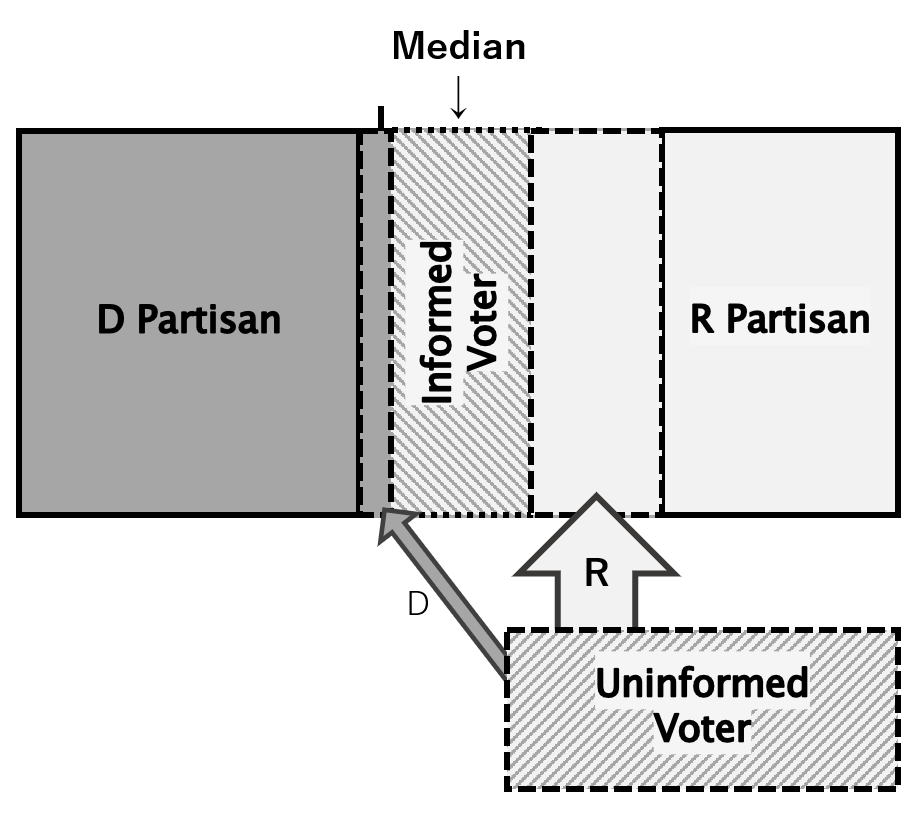
\includegraphics[width=70mm]{pictures/delegation_paper.png}
            \end{center}
            \caption{Delegation Logic}
            \label{delegation}
        \end{minipage}
        \begin{minipage}{0.5\hsize}
            \begin{center}
                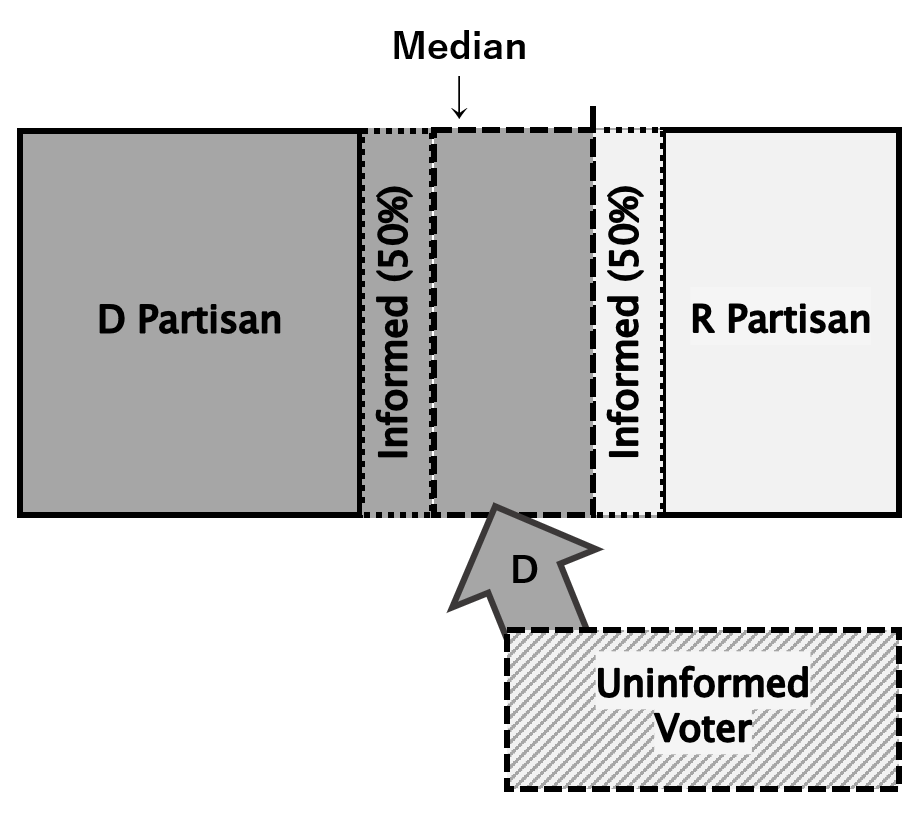
\includegraphics[width=70mm]{pictures/bandwagon_paper.png}
            \end{center}
            \caption{Bandwagon Logic}
            \label{bandwagon}
        \end{minipage}
    \end{figure}
    
    \subsection{Delegation}
    
    \par \cite{Feddersen1996thsw} introduce the first formal model to describe the logic of delegation. They categorize voters in the society into partisans, informed independents, and uninformed independents, and explains the behavior of each type of voters. Through the equilibrium analysis, they show that informed independents and partisans vote on their individual preference, but uninformed voters act so that they can ``maximize the probability that the informed independent agents determine the winner'' (414). To achieve this purpose, uninformed independents would participate in the election only when there is a partisan imbalance in the society, and when participating, they vote only to offset the partisan imbalance. As a result, uninformed voters can maximize the likelihood of votes by informed independents to determine the outcome of the election. 
    
    \par \autoref{delegation} illustrates this result in a more intuitive way. Suppose that there are two candidates from Party $D$ and Party $R$ in the election. As in any election, the outcome is determined by the majority. Thus median voter of the society determines the winner. $D$ partisan and $R$ partisan are those voters who are deeply identified with the corresponding party so that they always vote for their own party. On the other hand, informed voters and uninformed voters are neutral to the party (i.e., independents) and are interested in the qualitatively \textit{better} candidate. Informed voters know which candidate is better thus vote for the better candidate, while uninformed voters don't know which candidate is better. The \textit{delegation} logic suggests that knowing that they share preference with informed voters, uninformed voters distribute their votes to offset the partisan imbalance of the society. In the figure, $D$ partisan population is larger than $R$ partisan population. Thus uninformed voters distribute more votes to $R$ than $D$. As a consequence, the median voter of the society becomes informed voters, and thus the electoral outcome will be determined in favor of uninformed voters.  
    
    \subsection{Bandwagon}
    
    \par In contrast to the logic of delegation, the logic of bandwagon suggests that voters gain positive expressive benefit from voting with the expected majority of the society. Therefore, under the context of \autoref{bandwagon}, uninformed voters with bandwagon logic vote for Party $D$, which has a larger population of partisan than Party $R$. Under this logic, the votes of informed (independent) voters are just random noise in determining the expected majority in the society. There are numbers of rationales behind why bandwagoning behavior should occur \citep{Morton2015whmo, Tyran2016exev}. First set of mechanisms focuses on the psychological response to the social information \citep{Hardmeier2008thef}. Among them, \textit{contagion} implies the natural instinct to join the masses and \textit{gratification} focuses on the ``feels good'' aspect of to join in the winner side. Also, people may takes cues from social motivation to follow \textit{conformity} or \textit{consensus}. \textit{Self-persuasion} is a little more involved psychological response to convince oneself that the majority opinion is the ``right'' opinion. Another set of studies argues for the motivation to maximize the impersonal utility \citep{Coate2004grru, Feddersen2006thof, Feddersen2006thca}. 
    
    \par While it is not the intention of the current paper to specify the mechanism of bandwagoning, it can be expected that voters lacking the knowledge of their own preference are more susceptible to the non-preference-based, non-personal motivations for voting than informed voters. For example, the experiment conducted by \cite{Huckfeldt2014nobi} suggests that informed voters who obtained private information about their preference hold more durable opinions than uninformed voters who obtained no private information. Their study also shows that, compared to uninformed voters, informed voters are affected less by the social information obtained through the communication with others. Also, \cite{Roy2015anex} shows that the bandwagoning effect of social information is moderated by the depth of candidates information. They design mock election over a survey where respondents can search for information about candidates and provide the result of election polling random subset of respondents. The results suggest that those who searched more information about candidates (i.e., informed voters) are less likely to vote for the leading candidate in the polling than who did not search information (i.e., uninformed voters). 
    
    %\subsection{Conditions of Social Information Logic}
    
    %\par This paper has two theoretical propositions. First, it is suggested that social information is more influential in explaining uninformed voting behavior than informed voting behavior. The logic of the relationship between social information and voting behavior imply that social information is useful only among voters with high uncertainty in their preference. Second, I argue that the explanatory powers of two logic may differ across social information of different scales. The \textit{scale} here indicates the size of society in which the social information is extracted from. 
    
    %The scale ranges from as large as the nation to as small as counties. In explaining the interaction between the logic of uninformed voting and social information scales, first, the delegation logic is potentially the most applicable to the social information at the scale of the electoral district. Since uninformed voters under this logic primarily concerned with who is determining the electoral outcome, offsetting the partisan imbalance in the smaller scale than the electoral district does not help to achieve their goal. For example, if the election occurs at the scale of a nation (e.g., presidential election), delegation behavior may also occur against the national scale social information; if the election occurs at the scale of sub-national districts (e.g., Congressional election), delegation behavior should most likely be seen in the sub-national scale. On the other hand, the bandwagon logic often assumes that social information comes from close and visible society. To gain extra expressive benefit from following the majority of the particular society, the logic often requires close identification with that society.  Therefore it may make sense to expect that the bandwagoning logic is more applicable to the social information of smaller scales than larger scales.
    
    \section{Hypotheses}
    
    \par The hypotheses in this study is twofold. The first set of hypotheses focuses on the \textit{difference} in the logic of informed and uninformed voting: 
    
    \begin{verse}
        H1a: The less informed voters are, the more strongly social information explains their voting decisions. 
    \end{verse}
    \begin{verse}
        H1b: The less informed voters are, the less strongly individual preferences explain their voting decisions. 
    \end{verse}
    
    \noindent H1 suggests that social information is more influential in explaining uninformed voting behavior than informed voting behavior. The logic of the relationship between social information and voting behavior imply that social information is useful only among uninformed voters. Instead of relying on their uncertain preferences, uninformed voters refer to the social information to inform their decisions. The same logic does not apply to informed voters because they hold sufficient knowledge to form certain individual preferences.
    
    \par The second and third hypotheses concern the logical connection between social information and uninformed voting:
    
    \begin{verse}
        H2: In response to the social information, uninformed voters systematically vote against the majority (\textit{delegation}). 
    \end{verse}
    
    \begin{verse}
        H3: In response to social information, uninformed voters systematically vote for the majority (\textit{bandwagon}).
    \end{verse}
    
    \par H2 and H3 capture the competing logic of \textit{how} can social information influence uninformed voting. The analysis section of this paper explores the applicability of each logic. %may change across scales of social information.  The large-scale social information implies the information aggregated at national or state levels, and the small-scale social information implies the information aggregated at a county or smaller levels.
    
    %    \noindent As discussed in the last subsection of the theory section, comparing the predictive power of SVC model and BW model. BW model should have stronger predictive power in response to the social information with smaller scales.
    %
    %    \begin{verse}
    %        H3: The predictive power of H2b is stronger regarding the society of smaller scales, while the predictive power of H2a is stronger regarding the society of larger scales.
    %    \end{verse}
    
    \section{Research Design}
    
    % \subsection{Dataset}
    
    \par The current paper tests hypotheses by studying both presidential and congressional elections in the United States. Specifically, I use Cooperative Congressional Election Studies conducted in 2008 and 2016 (CCES2008 and CCES2016) and the history of presidential and congressional election outcomes aggregated at sub-national levels (i.e., county, congressional district, and state). The social information data are obtained from CQ Press Voting and Election Collections.\footnote{\url{http://library.cqpress.com/elections}. Accessed through the subscription of the library of the University of California, Davis.} The final dataset merges two data by the residential county, congressional district, and state of each CCES respondent's residence. 
     
    \par There are two advantages to use CCES for the analysis of this paper. First, the dataset includes a rich number of respondents from different locations across the United States, providing sufficient variations and data points in both county and state level social information. Second, the data are collected at the time of real-world election from a general population. The design of the study helps to generalize the findings to have real-world implications. It should be noted that the respondents of CCES are recruited from online and not nationally representative. The analysis uses sampling weights provided by the CCES organizers to correct for the potential bias in sampling.\footnote{Since the analysis includes the post-election variable of vote choice, post-election weights are used for CCES2016. General weights are used in CCES2008 because post-election weights are not provided.} Principal investigators of CCES do validate their sampling procedure by confirming that most of the actual election results do fall within the 95\% confidence interval of the estimates from CCES samples \cite{Ansolabehere2011guto, Ansolabehere2017guto}.  
    %Therefore, the absolute values from the analysis may not be representative of the American population. The discussion of this paper focuses on the relative behavior of informed voters and uninformed voters, not the absolute behavior of uninformed voters.
    
    % \par For the purpose of this paper, the dataset in the analysis only includes respondents who hold \textit{no} clear partisanship\footnote{More specifically, the analysis includes only those who consider themselves as neither Republican or Democrat.}. There are two justifications for this treatment. First, studies on voting behavior suggest that party identification plays a primal role in determining voting decisions \citep{Campbell1980tham,Lau2006hovo}. \cite{Achen2016defo} suggest that party identification can even influence the belief about political facts. Therefore, with clear identification of the party, the knowledge about neutral political facts may not be necessary to guide decisions in the election with partisan candidates. Second, moderate voters are often more influential in determining the electoral outcome than partisan voters. While partisan voters often hold the stable preference that is fixed across time, moderate voters ' preferences over candidate may swing across elections, thus affecting who wins elections. The analysis of this paper focuses on the moderate voters to isolate the role of information and deepen understanding of the voter population that is critical in determining electoral outcome.
    
    %     provides identifiers of residence at the country level. Using residential location data, the district environment variable of multiple scales (i.e., county and state) are reconstructed by linking each respondent with the regional level past voting patterns extracted from CQ Press Voting and Election Collections (\url{http://library.cqpress.com/elections/}). In addition to county and state level social information, the UC Davis module of the CCES 2016 comes with the information about the social network of each respondent. Thus, the first dataset involves three levels of social information: personal social network, residing county and state.
    
    %    \par In addition to CCES 2016, datasets with similar structure are under consideration, including American National Election Studies and other public opinion surveys that comes with social network modules. The alternative datasets would be used for the comparison and validation purposes regarding the findings from CCES 2016 dataset.
    
    \subsection{Variables and Model}
    
    \par The primary dependent variables for this study are the voter's choice of presidential and congressional (i.e., House of Representatives) candidates in 2008 and 2016 elections. Given that only a few voters vote for third party or independent candidates, this study focuses on the binary choice between Republican and Democratic candidates.\footnote{The votes to third-party candidates are considered as missing.} 
    
    \par To explain the dichotomous vote choice, four sets of predictors are relevant to this study. First, the measure of \textit{political knowledge} is constructed by the aggregation of eight factual test questions in CCES concerning the knowledge of the majority party in legislatures and party name of incumbent politicians. The correct answers are simply aggregated to construct the information scale (the Cronbach's alpha is 0.84 in 2008, 0.87 in 2016). The final score is normalized between 0 and 1.  
    
    \par Second, the measures of \textit{social information} are constructed by linking the aggregated electoral outcomes of past elections with each respondent in CCES. Past electoral outcomes may not be the direct representation of the partisan composition of the society, but the evident pattern in the past elections gives a strong cue as to how partisan preferences are distributed within society. From CQ Press Voting and Election Collections, I collect county and state level outcomes of presidential elections and congressional district and state level outcomes of congressional (i.e., House of Representatives) elections. Using two party Republican vote share in each subnational-unit, the versions of Partisan Voter Index (PVI) suggested by the Cook Political Report\footnote{\url{https://www.cookpolitical.com/pvi}} are calculated. State level PVI uses the following formula for each state $i$ and election cycle $t$: 
    \begin{align*}
    \textit{[State PVI]}_{t,i} = \{ & (\textit{[State Republican Share]}_{t-1, i} - \textit{[National Republican Share]}_{t-1}) + \\  
    &(\textit{[State Republican Share]}_{t-2, i} - \textit{[National Republican Share]}_{t-2}) \}/2
    \end{align*}    
    \noindent In the above formula, $t$ represents the current election and $t-1$ and $t-2$ represent the previous two elections. $\textit{[State Republican Share]}_i$ indicates two-party vote share of the Republican party against Democratic party in state $i$. Thus, \textit{State PVI} represents the average advantage of Republican party vote share over Democratic party relative to the national tendency in the previous two elections. The positive scores indicate the advantage in Republican vote share in percentage points, and the negative scores indicate the advantage in Democrat vote share in percentage points. The state-level measures are calculated for both presidential and congressional election vote shares.\footnote{Original PVI only concerns with presidential election vote share, but considering the measure's relevance for each election, I construct congressional election based measures for congressional election analysis.} In addition, county (for presidential election) or congressional district (for congressional election) level PVI measures are calculated using the following formula:
    \begin{align*}
        \textit{[County/District }&\textit{PVI]}_{t,i,j} = \\
        \{ &(\textit{[County/District Republican Share]}_{t-1, j} - \textit{[State Republican Share]}_{t-1,i}) + \\  
        &(\textit{[County/District Republican Share]}_{t-2, j} - \textit{[State Republican Share]}_{t-2, i}) \}/2
    \end{align*}    
    \noindent Notice that the above formula adjusts the PVI for county or congressional district $j$ not by national level vote shares but by state level vote shares. Therefore, the measure captures the partisan deviation of each county or congressional district from the state level average tendency. Due to this nature, the correlations between state and county or district PVI are very low (ranges from $-0.01$ to $0.14$), and it makes sense to include both variables into one model.
    % (-0.086 for 08 county,  -0.01108314 for 08 district  -0.04256889 for 16 county -0.1421199 for 16 district)
    
    %\par In addition to county and state level social information, 2008 and 2016 elections provide significantly different electoral environments in terms of national-level social information. While the 2008 election is conducted after the two consecutive winning of Republican candidates in the past two elections, 2016 election is conducted after the two consecutive winning of Democratic candidates in the past two elections. Therefore, national level social information may suggest Republican as the majority in the 2008 election and Democrat as the majority in 2016 election. One should be cautious about the generalizability of the above implication, but the subsequent analysis also looks at the general difference in the gap between uninformed and informed voters in 2008 and 2016 elections.
    
    \par The third and fourth set of predictors are included as controls. Those predictors relate to \textit{individual preference/evaluation} and \textit{demography} of voters. The individual preference/evaluation predictors include ideological closeness to candidates, leaning party\footnote{Note that clear partisanship holders are dropped from the analysis.}, and retrospective economic evaluation. Those attitudinal predictors are expected to be useful in explaining the decision of informed voters, but not uninformed voters. Lastly, the demographic variables include gender, age, race, education, and religiosity. All of those variables are either centered at median or set mode as 0 (if the variable is dichotomous). This paper has no specific expectations regarding how demographic variables interact with political knowledge, but those variables are included in the analysis to control for the baseline tendency in voting behavior.  
    
    \par Since the dependent variable of interest is the binary variable; I use logistic regression to estimate the impact of predictors on vote choice (Democrat = 0, Republican = 1). Population weights are used to weight cases to allow as much generalization as possible, and standard errors are clustered by states to incorporate common behavioral tendencies within states. The predictive model intends to identify the different behavioral patterns of informed and uninformed voters in response to social information, individual preferences and demographic characteristics.  This paper follows the approach taken by \cite{Bartels1996unvo} to include the complete set of linear interaction between each set of predictors and political information. The final model looks like follows:
    \begin{align*}
    Pr&(\text{Vote Republican})_i = \Lambda\{\\
    &\alpha + \beta (\text{Political Knowledge})_i +  \\
    &\delta_{1-2} (\text{Social Information})_i + \gamma_{1-2} (\text{Social Information})_i \times \text{Knowledge}_i + \\
    &\delta_{3-5} (\text{Individual Pref.})_i + \gamma_{3-5} (\text{Individual Pref.})_i \times \text{Knowledge}_i + \\
    &\delta_{6-10} (\text{Demographics})_i + \gamma_{6-10} (\text{Demographics})_i \times \text{Knowledge}_i \}
    \end{align*} 
    \noindent Assuming that there is a linear relationship between political information and predictive powers of each predictor, this method allows to estimate coefficients of each predictor at different levels of political information. Therefore, after the estimation, I calculate the conditional coefficients of each predictor for fully informed (political information $= 1$) and uninformed (political information $=0$) voters.
    
    %    \par The primary dependent variables for this study are voting decisions of individual voters. There are at least two ways to capture voting decisions. First is to use separate variables for voting participation (i.e., participate or not) and vote choice (i.e., which candidate to cast votes), and second is to use the unified variable for both participation and choice. If using the first approach, the logistic regression will be used to estimate the impact of social information on each of the dependent variable. This approach is simple and easy to interpret but fails to capture the direct connection between participation and vote choice decisions. The second approach will utilize multinomial logistic regression to assess the impact on participation and vote choice at the same time. This approach may complicate the interpretation of results but makes it possible to consider participation and vote choice decisions at the same time.
    
    %    \par In addition to estimation methods, this study considers multiple dependent variables from the same election. In particular, CCES 2016 has information about voting in presidential, senate, house, and state governor elections. It could be the case that voters use different behavioral rules in the different levels of elections. Therefore, the impact of social information is assessed for each level of elections.
    
    \section{Analysis}
    
\begin{knitrout}
\definecolor{shadecolor}{rgb}{0.969, 0.969, 0.969}\color{fgcolor}\begin{figure}[t!!!]

{\centering 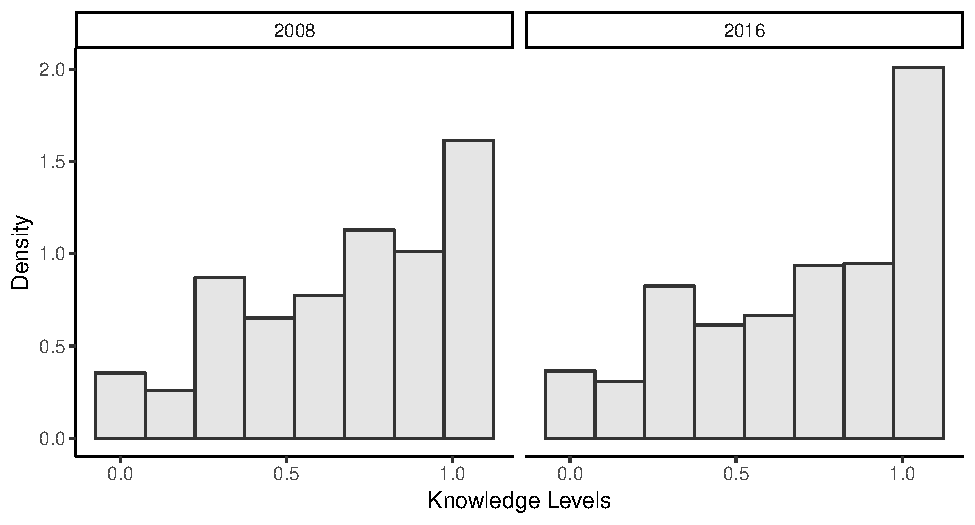
\includegraphics[width=\maxwidth]{figure/knidxgraph2-1} 

}

\caption[Distribution of Political Knowledge Scales]{Distribution of Political Knowledge Scales}\label{fig:knidxgraph2}
\end{figure}


\end{knitrout}
    
    \par Before starting the analysis, it is helpful to look at the descriptive distributions of two critical variables in this study: political knowledge and social information. To begin with, \autoref{fig:knidxgraph2} shows the distribution of political knowledge in datasets. It shows the large portion of respondents are fully informed of the factual questions offered in the survey (Knowledge levels = 1), while there are significant numbers of respondents who are uninformed or only partially informed. The distribution of knowledge is similar across 2008 and 2016 elections, while the 2016 election involves slightly more informed respondents. Given the nature of CCES as the online survey, it should be cautioned that the absolute distribution of knowledge may not be representative of the voters in the actual election. For this study, it just needed to be confirmed that there is a sufficient number of informed and uninformed voters to make a comparison of their behavioral patterns.  
    
\begin{knitrout}
\definecolor{shadecolor}{rgb}{0.969, 0.969, 0.969}\color{fgcolor}\begin{figure}[t!!!]

{\centering 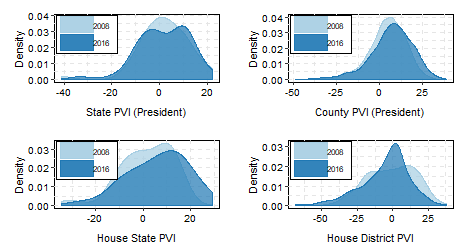
\includegraphics[width=\maxwidth]{figure/pvigraph2-1} 

}

\caption[Distribution of Social Information Variables]{Distribution of Social Information Variables}\label{fig:pvigraph2}
\end{figure}


\end{knitrout}
    
    \par Next, \autoref{fig:pvigraph2} shows the density distributions of social information variables. State level PVI are presented in left-hand panels and county and district level PVI are presented in right-hand panels. Those graphs show that the distributions of PVI are mostly single-peaked (with the slight exception in state PVI in 2016) and skewed to the left (there is a small number of units that are highly Democratic). It is also confirmed that significant variations exist in both state level and sub-state level PVI. Even when after adjusting for the level of partisan vote tendency in the state, county and district level PVI still have sufficient variance to explain vote choice. In fact, looking at the range of values in PVI, sub-state level PVI spread across a wider range of values than state PVI. 
    
\begin{knitrout}
\definecolor{shadecolor}{rgb}{0.969, 0.969, 0.969}\color{fgcolor}\begin{figure}[t!!!]

{\centering 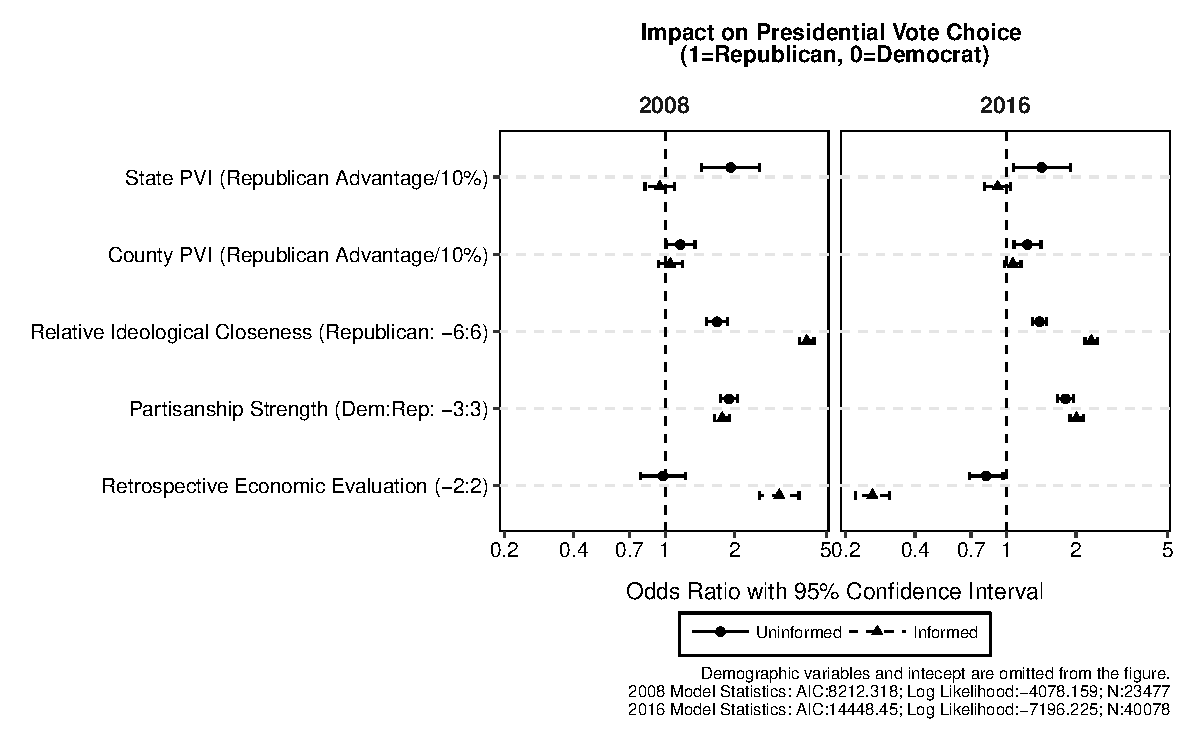
\includegraphics[width=\maxwidth]{figure/g2v_p-1} 

}

\caption[The Impact of Social Information on Informed and Uninformed Voting Behavior (Presidential Elections)]{The Impact of Social Information on Informed and Uninformed Voting Behavior (Presidential Elections)}\label{fig:g2v_p}
\end{figure}


\end{knitrout}
              
    \par The summary results for presidential election vote choice are presented in \autoref{fig:g2v_p}. Since all variables are interacted with knowledge index and the estimation is made by logistic regression, the plots show conditional coefficients for fully informed voters (political knowledge = 1) and uninformed voters (political knowledge = 0). To make the direct interpretation possible, the original coefficients are converted into odds ratio and presented with a 95 percent confidence interval. The coefficients of demographic variables are omitted from the plot (see Appendix for the detailed table). 
    
    \par The first and second rows of odds ratio plot shows the impact of social information on voting behavior. If H1a is correct, it should be seen that the odds ratio for uninformed voters is significantly more distant from the vertical line of 1 (which indicates null effect) than the odds ratio for informed voters. Consistent with this expectation, the state PVI odds ratio for uninformed voters is significantly more distant from 1 than the one for informed voters. In fact, in both 2008 and 2016 election, the impact of state PVI on vote choice is statistically significant (the 95 percent confidence interval does not cross 1) for uninformed voters, but not statistically significant for informed voters. The result for county PVI follows: county-level social information has a statistically significant impact ($p<.05$) on vote choice only among uninformed voters. 
    
    \par Regarding the direction of impact, the bandwagoning logic implies the positive relationship between PVI and the vote choice (odds ratio $> 1$), while the delegation logic implies the negative relationship between PVI and the vote choice (odds ratio $ < 1$). If H2 is correct, the impact of social information should be larger and above $1$, and if H3 is correct, the social information odds ratio must be smaller and below $1$. The result gives full support of H2 and rejects H3. This result implies that uninformed voters are \textit{bandwagoning} with the partisan majority in both counties and states. In both 2008 and 2016 presidential elections, 
    
\begin{knitrout}
\definecolor{shadecolor}{rgb}{0.969, 0.969, 0.969}\color{fgcolor}\begin{figure}[t!!!]

{\centering 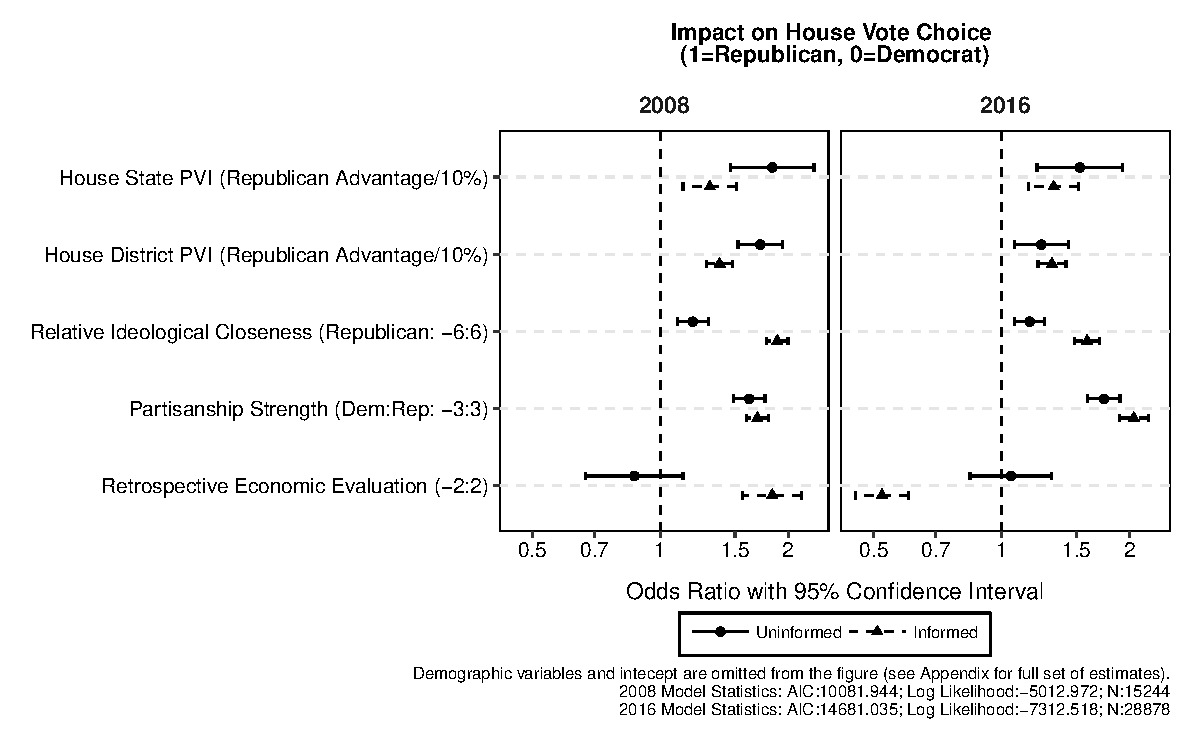
\includegraphics[width=\maxwidth]{figure/g2v_h-1} 

}

\caption[The Impact of Social Information on Informed and Uninformed Voting Behavior (Congressional Elections)]{The Impact of Social Information on Informed and Uninformed Voting Behavior (Congressional Elections)}\label{fig:g2v_h}
\end{figure}


\end{knitrout}
    
    \par Similarly, \autoref{fig:g2v_h} shows the results for congressional election vote choices. The implications follow that of presidential elections. However, the difference between uninformed and informed voters are smaller. To start with, social information in the House context have a statistically significant impact on vote choice of both informed and uninformed voters. On the other hand, social information variables have a stronger impact on uninformed choice than informed vote choice for all except for district PVI in 2016. In 2008, the difference between uninformed and informed voters is statistically significant ($p<.05$), while differences are not statistically significant in 2016. Overall, the congressional election results provide general but weaker support of H1a than presidential election results. 

    %\par For the role of national scale social information, the odds ratio of intercept can be potentially interpreted as the impact of national-level social information. Given that all the demographic variables are centered at the median, and individual preference/evaluation variables have $0$ as the neutral value, the relative difference in the intercepts implies the difference in the baseline likelihood of Republican votes for informed and uninformed voters with neutral social information and preferences/evaluations and median demographic characteristics. If H2 is correct, the delegation logic should be applied at the national scale. Thus, it should be seen that the intercept odds ratio for 2008 (when the social information implies Republican majority) is relatively smaller than the odds ratio for 2016 (when the social information implies Democratic majority). The result shows a consistent pattern with this expectation. In 2008, uninformed voters are relatively less likely to vote for McCain than Obama, and in 2016, uninformed voters are relatively more likely to vote for Trump than Clinton. 
    
    \par Regarding individual preference/evaluation variables, the result shows the consistent support of H1b in all elections. Ideological closeness and retrospective economic evaluation variables have relatively stronger explanatory power for informed voters than for uninformed voters in both 2008 and 2016 elections. The partisanship variable is an exception: it has similar levels of power to explain vote choice among both informed and uninformed voters. Overall, uninformed voters rely less on ideological preferences or retrospective evaluations to make voting decisions than informed voters, but party identity plays equally strong roles among informed and uninformed voters.
    
    \section{Simulating Aggregated Impact of Social Information}

    \par To gain deeper understandings of the significance of social information in uninformed voting, I conduct Monte Carlo simulation to assess the impact of social information on the aggregated outcome of vote choice. Since the estimated model includes a complex set of interacted variables, the simulation takes two steps. First, I estimate the predicted probability of vote choice for each respondent in surveys by only manipulating the values of social information (from 5 percentile to 95 percentile) and political knowledge (0 and 1). Values of other variables stay as it is. The uncertainty in predicted probabilities is also estimated by making each prediction 500 times, drawing random coefficient values generated according to the normal distribution with clustered standard error. Second, I aggregate predicted probabilities using population weights provided in CCES. This procedure gives an approximation of national level vote share for the given level of social information and knowledge. 

\begin{knitrout}
\definecolor{shadecolor}{rgb}{0.969, 0.969, 0.969}\color{fgcolor}\begin{figure}[t!!!]

{\centering 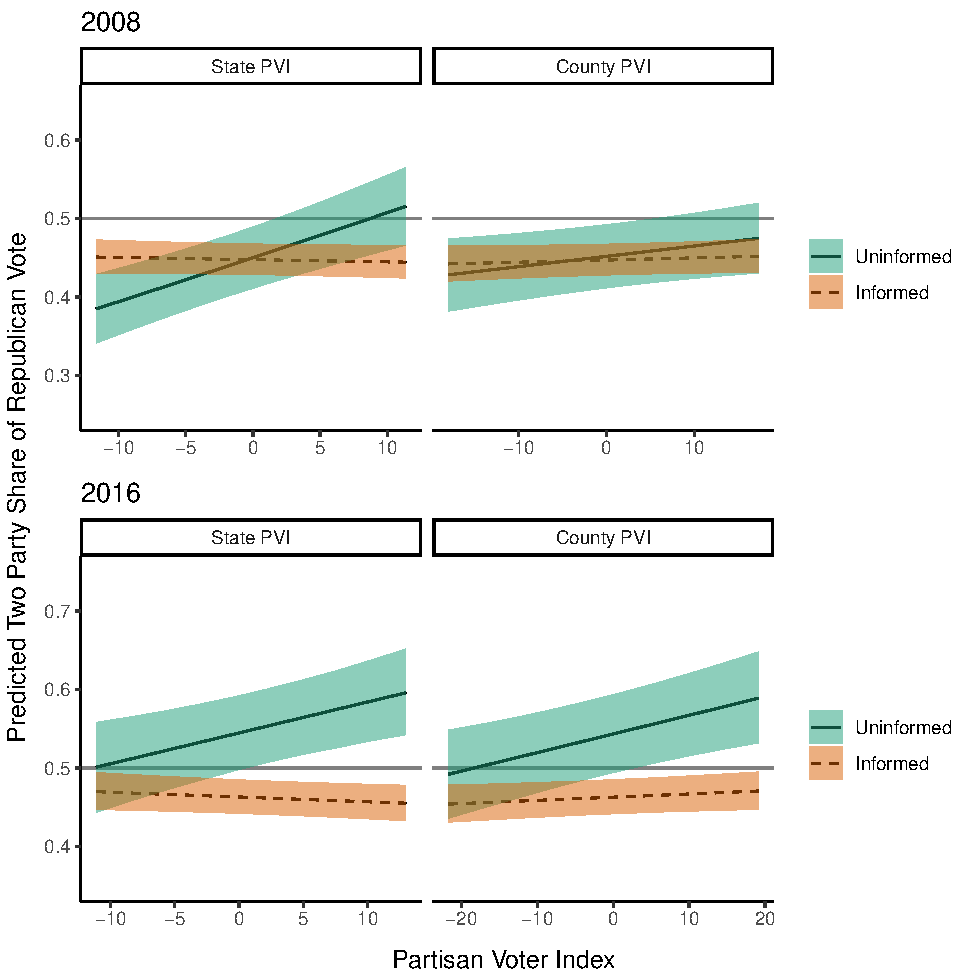
\includegraphics[width=\maxwidth]{figure/gagp2v_p-1} 

}

\caption[Only Uninformed Voters Bandwagon with Social Information (Presidential Elections)]{Only Uninformed Voters Bandwagon with Social Information (Presidential Elections)}\label{fig:gagp2v_p}
\end{figure}


\end{knitrout}
    
\begin{knitrout}
\definecolor{shadecolor}{rgb}{0.969, 0.969, 0.969}\color{fgcolor}\begin{figure}[t!!!]

{\centering 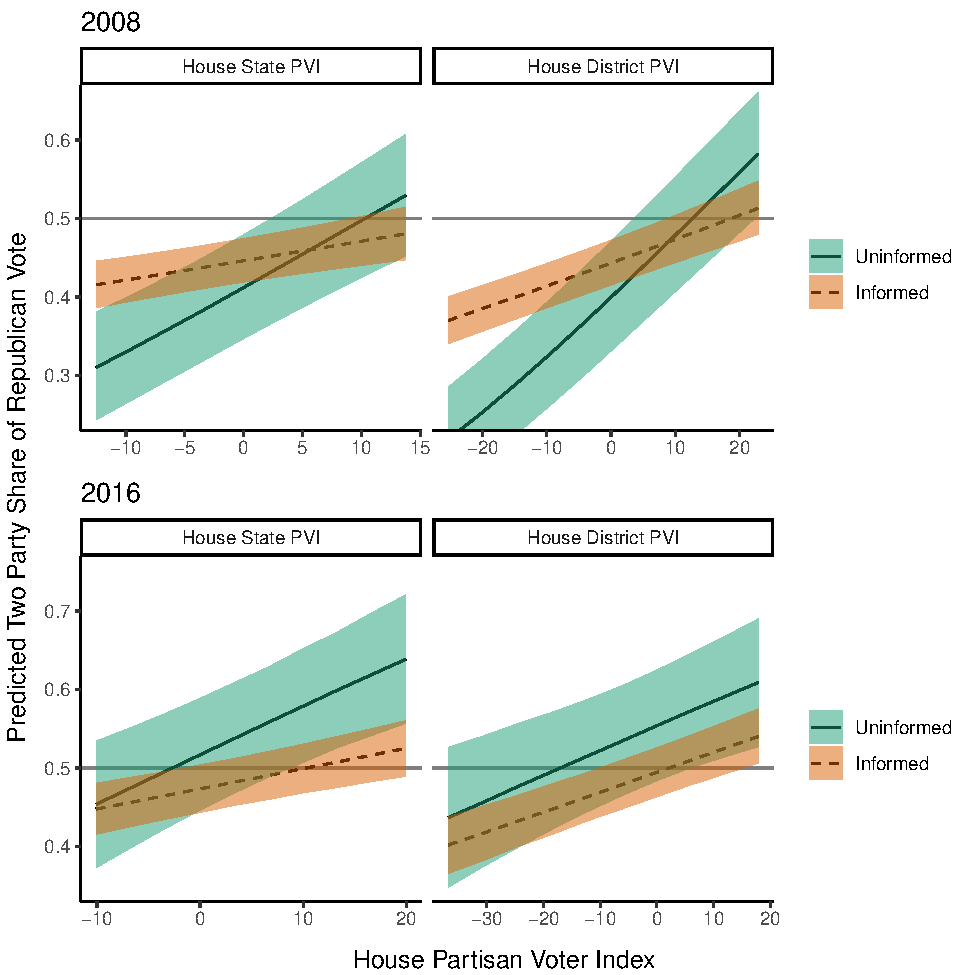
\includegraphics[width=\maxwidth]{figure/gagp2v_h-1} 

}

\caption[Uninformed Voters are More Strongly Pulled by Social Information Than Informed Voters (House Elections)]{Uninformed Voters are More Strongly Pulled by Social Information Than Informed Voters (House Elections)}\label{fig:gagp2v_h}
\end{figure}


\end{knitrout}
    
    \par \autoref{fig:gagp2v_p} plots the aggregated predicted share of the Republican vote in presidential elections as the function of social information and political knowledge levels. The shaded area represents 95\% confidence intervals in predictions. In both 2008 and 2016 elections, predicted Republican vote shares of fully informed voters stay almost constant across different values of social information. Also, note that predicted Republican shares for informed voters are significantly below 50\% in both elections (95\% confidence intervals does not cross 50\%). 
    
    \par In contrast, uninformed voters make a striking reaction to the values of social information. Especially in 2016, social information plays a significant role in raising the predicted uninformed vote share of Trump. The movement from 5 percentile to 95 percentile in state PVI and County PVI each correlates with 10-13\% increase in Republican vote share. Given the nature that the impacts of two PVI measures are additive, social information has a substantial effect in predicted uninformed electoral outcome. The impact of social information in 2008 election is somewhat weaker, but the predicted Republican share for uninformed voters increase from $38.4$\% to $51.7$\% when State PVI moves from 11.7\% Democratic advantage (5 percentile) to 11.4\% Republican advantage.

    \par \autoref{fig:gagp2v_h} presents the equivalent simulation for congressional elections. Here, it is easy to notice that social information, in general, plays a very strong role in determining vote choice. Even for informed voters, the higher score of state or district PVI correlate strongly with larger predicted share of Republican candidate. Uninformed voters do exhibit influence of social information in therir predicted vote share more strongly than informed voters. In 2008, the 5 percentile to 95 percentile movement in House Distrct PVI comes with more than 30\% increase in the predicted Republican share of uninformed voters, while for informed voters, the increase is limited to around 10\%.   

    \par The simulation of aggregated outcome illustrates the importance of taking social information into consideration when assessing the behavior of uninformed voters. Also notice that in 2016, there is an unexplained systematic difference between informed and uninformed voters: uninformed voters are predicted to vote more Republican even when PVI is fixed at 0. It is too early to conclude here, but this pattern may reflect the balancing behavior against the Democratic majority in previous elections. Further inquiry is needed for over-time comparison of uninformed voting.  
    
    \section{Discussion}
    
    \par Overall, the result of the analysis suggests that social information does play a significant role in explaining the behavior of uninformed voters, but not of informed voters (except for the county level social information in 2016 House election). This tendency gives consistent support of H1. Then, regarding the direction of impact of social information, the result gives strong support of bandwagon effect of voting with the majority of the society (H2), both in scales of state and county or congressional districts. This result partially supports the expectations of H2. H2 is supported in that uninformed voters apply delegation logic to the largest scale of social information. 
    
    \par Delegation hypothesis (H3) is rejected across all elections and social information considered in this paper. These results imply that strategic behavior of delegation behavior may not be occurring at the stage of vote choice. Here, at the stage of political participation, there have been several indicative empirical evidence that supports the proposition of strategic participation \cite{McMurray2010emev,Cantoni2017pras}. The result of the current paper suggests that it may be more fruitful for theoretical models of uninformed voting to consider participatory incentives than vote choice incentives of uninformed voters. 
    
    \par The result of this study provides evidence that informed and uninformed voters apply different logics in making vote choices using the dataset from the real-world election and general population sample. My result provide clues to answers the question proposed in the empirical studies of information effects: \textit{Why} information makes a systematic difference in the outcome of voting choices? The analysis of this study suggests that social information is one of the key variables to understand why informed and uninformed voter act in different ways. Using this result, the scholarly debate on civic competence can move forward from asking how illogical uninformed voters are to how the logic of uninformed voting affects the electoral outcomes. 
    
    \par There are at least two caveats to the result of this study. First, it should be noted that this study focuses on two recent presidential election years in the United States, and it is not clear if it can be generalized outside of those two elections. For example, it may be the case that voters exhibit different types of behavior mid-term election years. Further exploration is needed for this point. Second, the measurement of social information may have an issue of visibility. Theoretically, voters must observe the social information to use it for their decision-making. However, the objective measure of social information used in this study does not ensure that the information is observed by the respondent. Further study should explore whether presented social information is truly visible to voters. 
    
    \par In the future steps of this project, I intend to extend the current analysis into two directions. First, I intend to design the mock election experiment to test the more detailed mechanisms of the interaction between social information and uninformed voting behavior. The current analysis implicitly assumes the static, one-shot encounter to the social information, but the process of social information communication is more dynamic in the real world. The experiment would be useful in revealing the dynamic nature of social communication process. Second, I can use the current findings to construct the formal model of uninformed voting behavior. Recent development in formal studies suggests that information may not be the necessary factors for ``good'' democratic decisions \citep{Ashworth2014isvo}. By embedding the supposed behavioral rule of uninformed voters, the equilibrium analysis using the formal model will reveal the consequences of uninformed voting logic to the welfare of the society. The result will have a direct implication on the relationship between voter information and the quality of democracy.
    
    \clearpage
    % \theendnotes
    \singlespacing
    %\nocite{*}
    %\bibliography{C:/GoogleDrive/Reference/list_jabref.bib}
    \bibliography{uninformedchoice.bib}
    
    \clearpage
    \appendix
    \section{Detailed Table of the Estimation Result}
    
    \bigskip
    
    \scriptsize 

\begin{table}[h!!]
\caption{Impact on Presidential Vote Choice}
\begin{center}
\begin{footnotesize}
\begin{tabular}{l D{)}{)}{13)3} D{)}{)}{13)7} }
\toprule
 & \multicolumn{1}{c}{2008} & \multicolumn{1}{c}{2016} \\
\midrule
(Intercept)                                                   & -0.070 \; (0.230)       & 0.977 \; (0.155)^{***}      \\
Political Knowledge (0-1)                                     & 0.838 \; (0.337)^{*}    & -1.445 \; (0.223)^{***}     \\
State PVI (Republican Advantage/10\%)                         & 0.654 \; (0.148)^{***}  & 0.350 \; (0.145)^{*}        \\
County PVI (Republican Advantage/10\%)                        & 0.152 \; (0.074)^{*}    & 0.208 \; (0.069)^{**}       \\
Relative Ideological Closeness (Republican: -6:6)             & 0.518 \; (0.052)^{***}  & 0.329 \; (0.035)^{***}      \\
Partisanship Strength (Dem:Rep: -3:3)                         & 0.637 \; (0.043)^{***}  & 0.589 \; (0.041)^{***}      \\
Retrospective Economic Evaluation (-2:2)                      & -0.021 \; (0.116)       & -0.203 \; (0.085)^{*}       \\
Female                                                        & 0.021 \; (0.150)        & -0.845 \; (0.136)^{***}     \\
Age (by 10 years)                                             & 0.154 \; (0.045)^{***}  & 0.052 \; (0.036)            \\
Black                                                         & -4.621 \; (0.770)^{***} & -1.882 \; (0.336)^{***}     \\
Latino                                                        & -1.220 \; (0.304)^{***} & -1.236 \; (0.323)^{***}     \\
Asian                                                         & -0.168 \; (0.580)       & -0.976 \; (0.507)^{\dagger} \\
Other Race                                                    & -1.292 \; (0.473)^{**}  & -0.366 \; (0.331)           \\
Education (0-5)                                               & -0.107 \; (0.067)       & -0.092 \; (0.056)^{\dagger} \\
Born-Again Christian                                          & 0.429 \; (0.176)^{*}    & 0.722 \; (0.168)^{***}      \\
Knowledge * State PVI (Republican Advantage/10\%)             & -0.708 \; (0.188)^{***} & -0.442 \; (0.184)^{*}       \\
Knowledge * County PVI (Republican Advantage/10\%)            & -0.101 \; (0.111)       & -0.146 \; (0.097)           \\
Knowledge * Relative Ideological Closeness (Republican: -6:6) & 0.897 \; (0.073)^{***}  & 0.518 \; (0.049)^{***}      \\
Knowledge * Partisanship Strength (Dem:Rep: -3:3)             & -0.067 \; (0.068)       & 0.110 \; (0.056)^{\dagger}  \\
Knowledge * Retrospective Economic Evaluation (-2:2)          & 1.162 \; (0.192)^{***}  & -1.139 \; (0.138)^{***}     \\
Knowledge * Female                                            & 0.598 \; (0.222)^{**}   & 0.327 \; (0.200)            \\
Knowledge * Age (by 10 years)                                 & -0.028 \; (0.073)       & -0.052 \; (0.059)           \\
Knowledge * Black                                             & 2.321 \; (0.933)^{*}    & 0.445 \; (0.602)            \\
Knowledge * Latino                                            & 1.274 \; (0.502)^{*}    & 0.650 \; (0.615)            \\
Knowledge * Asian                                             & -0.973 \; (1.023)       & 0.527 \; (0.680)            \\
Knowledge * Other Race                                        & 2.026 \; (0.601)^{***}  & 0.611 \; (0.520)            \\
Knowledge * Education (0-5)                                   & -0.034 \; (0.087)       & -0.077 \; (0.067)           \\
Knowledge * Born-Again Christian                              & -0.029 \; (0.223)       & -0.203 \; (0.221)           \\
\midrule
AIC                                                           & 8212.318                & 14448.450                   \\
BIC                                                           & 8438.103                & 14689.211                   \\
Log Likelihood                                                & -4078.159               & -7196.225                   \\
Num. obs.                                                     & 23477                   & 40078                       \\
\bottomrule
\multicolumn{3}{l}{\tiny{$^{***}p<0.001$, $^{**}p<0.01$, $^*p<0.05$, $^{dagger}p<0.1$}}
\end{tabular}
\end{footnotesize}
\label{table:coefficients}
\end{center}
\end{table}


\begin{table}[h!!]
\caption{Impact on House Vote Choice}
\begin{center}
\begin{footnotesize}
\begin{tabular}{l D{)}{)}{13)7} D{)}{)}{13)7} }
\toprule
 & \multicolumn{1}{c}{2008} & \multicolumn{1}{c}{2016} \\
\midrule
(Intercept)                                                   & -0.537 \; (0.276)^{\dagger} & 0.449 \; (0.173)^{**}      \\
Political KNowledge (0-1)                                     & 0.997 \; (0.373)^{**}       & -0.714 \; (0.218)^{**}     \\
House State PVI (Republican Advantage/10\%)                   & 0.608 \; (0.115)^{***}      & 0.424 \; (0.119)^{***}     \\
House District PVI (Republican Advantage/10\%)                & 0.541 \; (0.061)^{***}      & 0.215 \; (0.074)^{**}      \\
Relative Ideological Closeness (Republican: -6:6)             & 0.176 \; (0.043)^{***}      & 0.152 \; (0.042)^{***}     \\
Partisanship Strength (Dem:Rep: -3:3)                         & 0.482 \; (0.043)^{***}      & 0.554 \; (0.045)^{***}     \\
Retrospective Economic Evaluation (-2:2)                      & -0.140 \; (0.134)           & 0.050 \; (0.113)           \\
Female                                                        & -0.080 \; (0.169)           & -0.123 \; (0.186)          \\
Age (by 10 years)                                             & 0.022 \; (0.055)            & -0.039 \; (0.051)          \\
Black                                                         & -2.346 \; (0.529)^{***}     & -1.532 \; (0.351)^{***}    \\
Latino                                                        & -0.337 \; (0.410)           & -1.002 \; (0.304)^{***}    \\
Asian                                                         & 0.690 \; (0.545)            & 0.234 \; (0.700)           \\
Other Race                                                    & -1.606 \; (0.502)^{**}      & -0.009 \; (0.461)          \\
Education (0-5)                                               & 0.029 \; (0.069)            & -0.112 \; (0.053)^{*}      \\
Born-Again Christian                                          & 0.165 \; (0.164)            & 0.311 \; (0.196)           \\
Knowledge * House State PVI (Republican Advantage/10\%)       & -0.339 \; (0.152)^{*}       & -0.142 \; (0.155)          \\
Knowledge * House District PVI (Republican Advantage/10\%)    & -0.220 \; (0.077)^{**}      & 0.058 \; (0.098)           \\
Knowledge * Relative Ideological Closeness (Republican: -6:6) & 0.458 \; (0.061)^{***}      & 0.312 \; (0.063)^{***}     \\
Knowledge * Partisanship Strength (Dem:Rep: -3:3)             & 0.044 \; (0.063)            & 0.161 \; (0.069)^{*}       \\
Knowledge * Retrospective Economic Evaluation (-2:2)          & 0.747 \; (0.181)^{***}      & -0.698 \; (0.154)^{***}    \\
Knowledge * Female                                            & 0.362 \; (0.221)            & -0.229 \; (0.243)          \\
Knowledge * Age (by 10 years)                                 & -0.054 \; (0.077)           & -0.009 \; (0.072)          \\
Knowledge * Black                                             & 1.914 \; (0.738)^{**}       & 1.199 \; (0.517)^{*}       \\
Knowledge * Latino                                            & 0.402 \; (0.558)            & 0.831 \; (0.429)^{\dagger} \\
Knowledge * Asian                                             & -1.595 \; (0.722)^{*}       & -0.453 \; (1.006)          \\
Knowledge * Other Race                                        & 1.815 \; (0.622)^{**}       & 0.411 \; (0.561)           \\
Knowledge * Education (0-5)                                   & -0.049 \; (0.091)           & 0.139 \; (0.073)^{\dagger} \\
Knowledge * Born-Again Christian                              & -0.219 \; (0.235)           & 0.197 \; (0.296)           \\
\midrule
AIC                                                           & 10081.944                   & 14681.035                  \\
BIC                                                           & 10295.639                   & 14912.619                  \\
Log Likelihood                                                & -5012.972                   & -7312.518                  \\
Num. obs.                                                     & 15244                       & 28878                      \\
\bottomrule
\multicolumn{3}{l}{\tiny{$^{***}p<0.001$, $^{**}p<0.01$, $^*p<0.05$, $^{dagger}p<0.1$}}
\end{tabular}
\end{footnotesize}
\label{table:coefficients}
\end{center}
\end{table}

    
\end{document}
